%=========================================================================
% sec-intro
%=========================================================================

\section{Introduction}
\label{sec-intro}

\begin{figure}[b]
  \begin{minipage}[b]{0.42\tw}
    %=========================================================================
% fig-intro-overview
%=========================================================================

%\begin{figure}

  \centering
  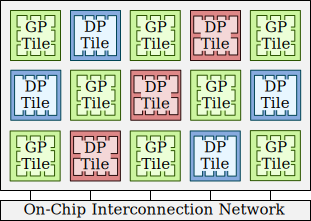
\includegraphics[width=\tw]{intro-overview.svg.pdf}

  \caption{\textbf{Example of Fine-Grain Heterogeneous Architectures --}
    A sea of lightweight compute tiles composed of both general-purpose
    tiles (CPUs) and accelerators specialized for exploiting varying
    forms of parallelism (GPUs for graphics and DSPs for digital signal
    processing).}

  \label{fig-intro-overview}

%\end{figure}

  \end{minipage}%
  \hfill%
  \begin{minipage}[b]{0.56\tw}
    %=========================================================================
% fig-intro-vision
%=========================================================================

%\begin{figure}

  \centering
  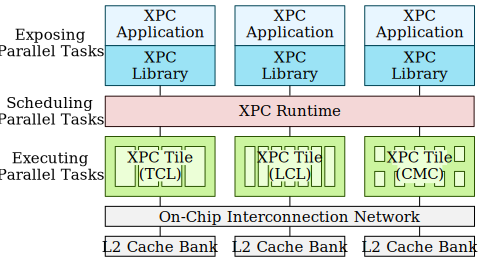
\includegraphics[width=\tw]{intro-vision.svg.pdf}

  \caption{\textbf{XPC Architecture Overview --} XPC applications use an
    XPC parallel programming library to expose fine-grain parallel
    tasks. A software runtime is used to facilitate adaptive task
    distribution to the available hardware resources based on collected
    heuristics. Heterogeneous XPC tiles are specialized for various forms
    of parallelism, but all XPC tiles have the same ISA.}

  \label{fig-intro-vision}

%\end{figure}

  \end{minipage}
\end{figure}

Microprocessor design has reached the limits of improving performance and
energy efficiency by scaling the number of general-purpose cores on a
chip. Instead, computer architects are turning toward a heterogeneous mix
of general-purpose cores and data-parallel accelerators to exploit the
ubiquitous data parallelism present in modern applications such as graph
processing, physical simulation, big data analytics, and machine
learning. Recent examples include the Intel
Haswell~\cite{hammarlund-intel-haswell-ieeemicro2014}, AMD
Kabini~\cite{bouvier-amd-kabini-ieeemicro2014}, and NVIDIA Tegra
4~\cite{krewell-nvidia-tegra4-mpr2013}, which integrate general-purpose
multicores with programmable graphics processing units (GPUs) at a coarse
granularity. Although this strategy has been promising, there is no clear
answer yet to the new challenges imposed by heterogeneous architectures,
like a unified software framework or optimal scheduling for adaptive
execution. In order to address these challenges, I believe the future
will move toward a more \emph{fine-grain intermingling} of many
lightweight general-purpose cores and data-parallel accelerators unified
under a single ISA with support for \emph{seamless adaptive execution} of
parallel tasks as shown in Figure~\ref{fig-intro-overview}.

Data-parallel accelerators like those used in current coarse-grain
heterogeneous architectures focus on exploiting \emph{conventional data
  parallelism} in which tasks generally have highly regular control and
memory-access structures and do not interact with each other.  However, a
growing number of modern applications exhibit a generalized form of data
parallelism called \emph{amorphous data parallelism} in which tasks can
conflict with each other, be generated dynamically, and modify the
underlying data structure~\cite{pingali-tao-pldi2011}. Mapping such
applications to current data-parallel accelerators can be difficult and
usually require aggressive software
optimizations~\cite{luo-gpu-bfs-dac2010,harish-large-graph-gpu-hipc2007,
  hong-cuda-max-warp-ppopp2011,nasre-data-vs-topo-ipdps2013,
  nasre-morph-ppopp2013,mendez-optimizations-amorphous-ppopp2010,
  mendez-gpu-pta-ppopp2012}. Ideally, future fine-grain heterogeneous
architectures would employ accelerators for a broader range of amorphous
data parallelism. These amorphous-data-parallel accelerators would be
specialized not only for varying degrees of irregularity, but also for
efficient conflict resolution or dynamic task generation. A broader range
of accelerators would provide more options for adaptively scheduling
tasks to accelerators they are best suited for.

This proposal outlines the Explicit-Parallel-Call (XPC) architecture, a
fine-grain heterogeneous architecture based on the concept of explicitly
encoding parallel tasks as parallel function calls in the software/hardware
interface. Figure~\ref{fig-intro-overview} highlights the vertically
integrated methodology that will be used to explore both software and
hardware techniques for \emph{exposing}, \emph{scheduling}, and
\emph{executing} fine-grain parallel tasks.

Several aspects of the XPC architecture are inspired by my previous work
on general-purpose graphics processing units (GPGPUs). In the paper
published at ISCA 2013, I was able to improve the performance and energy
efficiency of conventional data parallel applications GPGPUs by
exploiting a new form of structure called \emph{value structure} to
detect and eliminate redundant
computations~\cite{kim-simt-vstruct-isca2013}. The benefits of this
technique was less apparent for applications with more amorphous data
parallelism. This issue was addressed in the paper published at MICRO
2014, where \emph{hardware worklists} were utilized in GPGPUs to improve
memory contention and load balancing when managing fine-grain parallel
tasks, resulting in promising speedups for amorphous data parallel
applications~\cite{kim-hwwl-micro2014}. The insights from these studies
helped guide the designs for a broader range of data-parallel
accelerators and system-wide task distribution schemes.
